\section{实验步骤}
\subsection{实验准备}

在本次实验中,我直接采用实验二中的showStack.c(代码\ref{lst:launch})对应的可执行程序showStack.exe。

如代码\ref{lst:showStack}所示,为了调试内核代码部分,在lauch.json中将调试目标设置为Kernel.exe.

\begin{listing}[htbp]
    \begin{minted}{python}
"program": "${workspaceFolder}/target/objs/kernel.exe",
// "program": "${workspaceFolder}/target/objs/apps-elf/showStack",
    \end{minted}
    \caption{launch.json program配置部分}\label{lst:launch}
\end{listing}

\begin{listing}[htbp]
    \begin{minted}{c}
#include <stdio.h>
int version = 1;
int sum(int var1, int var2)
{
    int count;
    version = 2;
    count = var1 + var2;
    return (count);
}
void main1()
{
    int a, b, result;
    a = 1;
    b = 2;
    result = sum(a, b);
    printf("result=%d\n", result);
}
    \end{minted}
    \caption{showStack.c}\label{lst:showStack}
\end{listing}
\subsection{找到进程完整的图像}

按照实验指导,我在Process::Exit()函数中设置断点。如图\ref{showStack},\ref{hit}所示,
在远程桌面中运行showStack程序后,命中之前所设置的断点。此时,点击VARIABLES面板中的Locals栏里的u项来
查看User结构。特别地,如图\ref{proc}所示,我展开其中的u\_procp项来查看Proc结构。更进一步,我展开其中的p\_textp项来
查看Text结构。

\begin{figure}[!htbp]
    \centering
    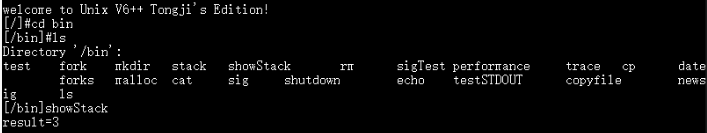
\includegraphics[width=\textwidth]{figures/showStack.png}
    \caption{运行showStack.exe}\label{showStack}
\end{figure}
\begin{figure}[!htbp]
    \centering
    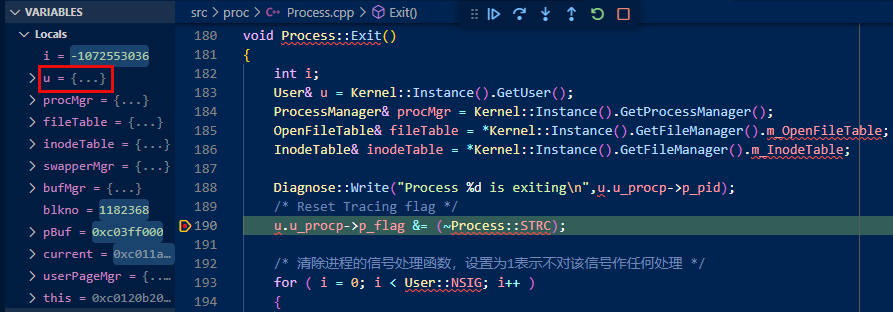
\includegraphics[width=\textwidth]{figures/hit.png}
    \caption{命中断点}\label{hit}
\end{figure}
\begin{figure}[!htbp]
    \centering
    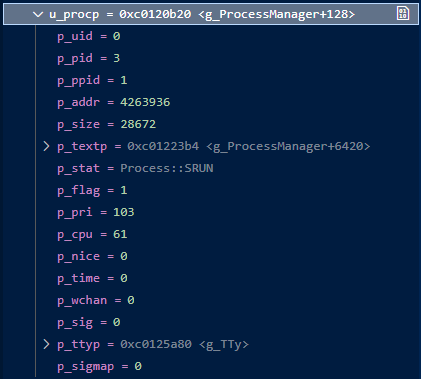
\includegraphics[scale=1]{figures/u_procp.png}
    \caption{查看Proc结构}\label{proc}
\end{figure}
\begin{figure}[!htbp]
    \centering
    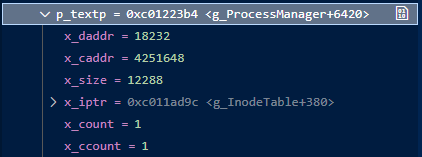
\includegraphics[scale=1]{figures/p_textp.png}
    \caption{查看Text结构}\label{text}
\end{figure}

表\ref{User}-\ref{Text}为上述三个结构体的对应说明。

通过右键点击Vscode中VARIABLE中的变量,并选择“Copy as Expression”,即可获得对应变量的访问方式。
通过这一方法,可以得到从User结构u出发,访问进程的代码段的起始位置的物理地址的方式为\verb|(((u).u_procp)->p_textp)->x_caddr|;
访问进程的可交换部分起始位置的逻辑地址的方式为\verb|((u).u_procp)->p_addr|。而User结构u则是通过\verb|Kernel::Instance().GetUser()|获得,
具体实现为返回常量3G+4M-4K。

对于代码段和可交换部分起始位置的逻辑地址,根据UNIX V6++的实现方式,我们可以直接给出:代码段起始位置的逻辑地址为4M+4K;可交换部分(PPDA区)起始位置的逻辑地址为8M-4K。
当然,代码段起始位置的逻辑地址也可以通过\verb|((u).u_MemoryDescriptor).m_TextStartAddress|获得。

更进一步,如表\ref{relative}和表\ref{directory}-\ref{table768}所示,可以根据现有的信息以及UNIX V6++的实现方法绘制出该进程的相对地址映射表和物理页表。

\subsection{找到进程的相对虚实地址映射表}

    通过执行exec命令视察内存空间,可以得到图\ref{relative_mem}中的结果,表\ref{relative_after}为在此基础上填写的实验指导中的表5。经过对比,该结果与表\ref{relative}一致。

\begin{Verbatim}[frame=single,fontsize=\small]
    -exec x /20xw 0xC0209004
    0xc0209004:	0x00000ffd	0x00001ffd	0x00002ffd	0x00001fff
    0xc0209014:	0x00002fff	0x00003fff	0x00004fff	0x00005fff
    0xc0209024:	0x00000ffc	0x00000ffc	0x00000ffc	0x00000ffc
    0xc0209034:	0x00000ffc	0x00000ffc	0x00000ffc	0x00000ffc
    0xc0209044:	0x00000ffc	0x00000ffc	0x00000ffc	0x00000ffc    
    -exec x /4xw 0xC0209FF0
    0xc0209ff0:	0x00000ffc	0x00000ffc	0x00000ffc	0x00006fff
\end{Verbatim}
\captionof{figure}{视察相对虚实地址映射表所在内存空间}\label{relative_mem}

\subsection{找到进程的物理页表}

由UNIX V6++的实现可知,与现运行进程相关的4张物理页表的逻辑地址分布在3G+2M-3G+2M+16K内,一张页表的大小为4K。

逻辑地址3G+2M-3G+2M+4K-1内装有一级页表。表\ref{directory_after}为对应表格。

\begin{Verbatim}[frame=single,fontsize=\small]
    -exec x /4xw 0xC0200000
    0xc0200000:	0x00202027	0x00203027	0x00000000	0x00000000
    -exec x /4xw 0xC0200C00
    0xc0200c00:	0x00201023	0x00000000	0x00000000	0x00000000
\end{Verbatim}
\captionof{figure}{视察一级页表所在内存空间}\label{relative_directory}

逻辑地址3G+2M+4K-3G+2M+8K-1内装有第768张二级页表。表\ref{page768_after}为对应表格。

\begin{Verbatim}[frame=single,fontsize=\small]
    -exec x /4xw 0xC0201000
    0xc0201000:	0x00000003	0x00001003	0x00002003	0x00003003
    -exec x /4xw 0xC0201FF0
    0xc0201ff0:	0x003fc003	0x003fd003	0x003fe003	0x00411063
\end{Verbatim}
\captionof{figure}{视察第768张二级页表所在内存空间}\label{mem768}

逻辑地址3G+2M+8K-3G+2M+12K-1内装有第0张二级页表。表\ref{page0_after}为对应表格。

\begin{Verbatim}[frame=single,fontsize=\small]
    -exec x /20xw 0xC0202000
    0xc0202000:	0x00000067	0x00404004	0x00404004	0x00404004
    0xc0202010:	0x00404006	0x00404006	0x00404026	0x00404006
    0xc0202020:	0x00404006	0x00404006	0x00404006	0x00404006
    0xc0202030:	0x00404006	0x00404006	0x00404006	0x00404006
    0xc0202040:	0x00404006	0x00404006	0x00404006	0x00404006
\end{Verbatim}
\captionof{figure}{视察第0张二级页表所在内存空间}\label{mem0}

逻辑地址3G+2M+12K-3G+2M+16K-1内装有第1张二级页表。表\ref{page1_after}为对应表格。

\begin{Verbatim}[frame=single,fontsize=\small]
    -exec x /12xw 0xC0203000
    0xc0203000:	0x00404006	0x0040e065	0x0040f065	0x00410065
    0xc0203010:	0x00412067	0x00413067	0x00414067	0x00415067
    0xc0203020:	0x00416067	0x00416066	0x00417066	0x00404006    
    -exec x /4xw 0xC0203FF0
    0xc0203ff0:	0x00404006	0x00404006	0x00404006	0x00417067
\end{Verbatim}
\captionof{figure}{视察第1张二级页表所在内存空间}\label{mem1}

经过对比,根据实验得到的4张页表与自行填写的四张页表一致。